% ================================================================================================
\documentclass[8pt, a4paper, twoside]{extarticle}
%\documentclass[fontsize=8pt, a4paper, fleqn, landscape, DIV=calc]{scrartcl}
% Font size:    8pt
% Paper size:   A4
% style:        twoside (needed, so odd and even pages have different margins)

% ========================================= DOCUMENT INFO =========================================
\def\title{Elektrochemie}           					                            % title
\def\shorttitle{ElChem OST} 								                        % short title (displayed as PDF title)
\def\dozent{Mario Graf}         		                                            % lecturer
\def\semester{FS 2025} 									                            % semester
\def\author{Fabian Suter \& Steiner,  \\ Vorlage: Yves Looser, Nino Briker, Sandro Heidrich}  	% author(s)
\def\repo{https://github.com/FabianSuter/ElChem.git} % TODO: Check                  % repository link
\def\version{0.0.1}   										                        % version
\def\pagelimit{10}           								                        % page limit -> causes pages after limit to be red
\def\titleoption{normal}   									                        % options: compact, normal
\def\enableToC{true}

% ================================= PACKAGES, SETUP AND COMMANDS ==================================
% =========================================== PACKAGES ============================================
\usepackage[utf8]{inputenc}         % input encoding: UTF-8
\usepackage[T1]{fontenc}            % font encoding: T1
\usepackage{textcomp}               % additional symbols
\usepackage{times}                  % times new roman font
\usepackage[main=ngerman]{babel}    % set main language to german


\usepackage{multicol}               % provides multicols environment
\usepackage{multirow}               % provides multirow environment
\usepackage{geometry}               % set page layout


\usepackage{enumitem}               % list customization
\usepackage{outlines}               % easy nested lists
\usepackage{tabularx}               % some nicer tables with X columns
\usepackage{hhline}                 % double lines in tables
\usepackage{booktabs}               % thick and thin lines in tables


\usepackage{amsmath}                % math symbols
\usepackage{amssymb}                % more math symbols
\usepackage{mathtools}              % more math tools needed for pmatrix modification
\usepackage{mhsetup}                % needed to modify pmatrix environment
\usepackage{txfonts}                % Times math font
\usepackage[squaren]{SIunits}       % SI-units
\usepackage{bm}                     % bold math symbols
\usepackage{trfsigns}               % needed for "Laplace" symbol (Korrespondenz)
\usepackage{mathrsfs}               % needed for Fourier transform "F"


\usepackage{graphicx}               % include graphics
\usepackage{graphbox}               % needed for aligning images in multicol environment
\usepackage{scalerel}               % scale any objects
\usepackage{anyfontsize}            % set any font size
\usepackage{xcolor}                 % needed for colors
\usepackage[table]{xcolor}          % needed for special colors in tables
\usepackage{stackengine}            % TODO: check if needed, For stacking objects


\usepackage{tcolorbox}              % colored boxes
\usepackage[outline]{contour}       % contour for text (used in custom underline command)
\usepackage[normalem]{ulem}         % custom underline (used in custom underline command)


\usepackage{tikz}                   % needed for TikZ drawings


% \usepackage{listings}               % for nicer code display
% to use nodes inside listing see: https://texample.net/tikz/examples/tikz-listings/


\usepackage{hyperref}               % clickable links
\usepackage{qrcode}                 % QR code generation (also clickable)


\usepackage{ifthen}                 % if-then-else commands
\usepackage{calc}                   % simple arithmetic in LaTeX commands


\usepackage{draftwatermark}         % watermark on pages after a certain limit
\usepackage{fancyhdr}               % custom header and footer
\usepackage[explicit]{titlesec}     % custom section titles


\usepackage{datetime2}              % custom date format for versioning


\usepackage{chemfig}                % For drawing molecules with TikZ
\usepackage{chemformula}            % Command for typesetting chemical formulas and reactions
\usepackage{elements}               % For data of chemical elements, until 112
\usepackage[version=4]{mhchem}      % For  chemical molecular formulae and equations


% ========================================== BASIC SETUP ==========================================

% --------------------------------------- DOCUMENT SETTINGS ---------------------------------------
\hypersetup{hidelinks,
% set pdf metadata
            pdfauthor={\author},
            pdftitle={\shorttitle},
            pdfsubject={\title\ \semester},
            pdfkeywords={Gahn go lerne!!}}

% set style for URLs
\urlstyle{same} % sets url font to the same as the preceeding text

% set page layout
\geometry{left=3mm, 
          right=3mm, 
          top=3mm, 
          bottom=6mm, 
          headheight=0mm, 
          headsep=0mm, 
          footskip=4mm}

\setlength{\columnsep}{1.5mm}       % distance between columns
\setlength{\columnseprule}{0.1pt}   % thickness of column separation line
\setlength{\parindent}{0pt}         % no paragraph indentation

\setcounter{tocdepth}{2}            % only display sections and subsections in toc
% \setcounter{secnumdepth}{0}       % uncomment to disable section numbering

\DeclareMathSizes{8}{8}{6}{5}       % set math font sizes for 8pt document


% --------------------------------------- COLOR DEFINITIONS ---------------------------------------
\definecolor{sectioncolor}{RGB}{255,100,0}
\definecolor{subsectioncolor}{RGB}{255,200,0}
\definecolor{sectextcol}{RGB}{255,255,255}
\definecolor{subsectextcol}{RGB}{0,0,0}

\definecolor{backcolour}{HTML}{f5f5f0} % background color for highlighted text

% TODO: define color palette
% color palette: https://colorkit.co/color-palette-generator/FF8552-9e22bd-404E7C-C32E15-225A28/
\definecolor{green}{HTML}{1af430}
\definecolor{red}{HTML}{f90d09}
\definecolor{blue}{HTML}{093ce5}
\definecolor{orange}{HTML}{f7730e}
\definecolor{violet}{HTML}{a516c9}

% colors for listings (code)
% \definecolor{commentcolour}{HTML}{404E7C}
% \definecolor{keywordcolour}{HTML}{225A28}
% \definecolor{stringcolour}{HTML}{9e22bd}
% \definecolor{numbercolour}{HTML}{808080}


% ----------------------------------- LIST AND TABULAR SETTINGS -----------------------------------
\setlist[enumerate]{%
    labelindent=0pt,                                % no indentation for labels
    labelwidth = \widthof{\ref{enum-\EnumitemId}},  % set label width to widest label
    label=\bfseries\arabic*.,                       % label style bold arabic numerals (1., 2., ...)
    itemindent=1ex,                                 % separation between label and item text
    leftmargin=!,                                   % automatically calculate left margin
    after=\label{enum-\EnumitemId}}                 % set label for referencing in labelwidth

\setlist[itemize]{leftmargin=1.5em}                 % left margin for itemize: 1.5em
\setlist{nosep}                                     % no vertical spacing between list items

\renewcommand{\arraystretch}{1}                     % stretch table rows

\setcounter{MaxMatrixCols}{32}                      % increase max columns in matrix environments

% ----------------------------------------- TIKZ SETTINGS -----------------------------------------
\usetikzlibrary{arrows}
\usetikzlibrary{arrows.meta}
\usetikzlibrary{bending}
\usetikzlibrary{decorations.pathreplacing}
\usetikzlibrary{angles}
\usetikzlibrary{tikzmark}
\usetikzlibrary{petri}
\usetikzlibrary{positioning}
\usetikzlibrary{shapes}
\usetikzlibrary{calc}


% ------------------------------------ OTHER PACKAGE SETTINGS -------------------------------------

% define and set new date style for versioning as YYYYMMDD
\DTMnewdatestyle{vnumdate}{%
    \renewcommand{\DTMdisplaydate}[4]{\number##1\DTMtwodigits{##2}\DTMtwodigits{##3}}%
    \renewcommand{\DTMDisplaydate}{\DTMdisplaydate}%
}
\DTMsetdatestyle{vnumdate}


% setup for ulem and contour packages
\renewcommand{\ULdepth}{1.75pt} % set underline depth
\contourlength{0.7pt}           % set contour length


% ====================================== SETUP AND COMMANDS =======================================

% custom underline command for exclusions on lowercase letters such as g, j, p, q, y
\newrobustcmd{\myul}[1]{%
    \uline{\phantom{#1}}%
    \llap{\contour{white}{#1}}%
}

\renewrobustcmd{\underline}[1]{%
    \uline{\phantom{#1}}%
    \llap{\contour{white}{#1}}%
}


% setup header and footer
\pagestyle{fancy}
\fancyhf{}                          % clear all header and footer fields
\renewcommand{\headrulewidth}{0pt}  % remove header rule
\renewcommand{\footrulewidth}{0pt}  % remove footer rule
\fancyfoot[C]{\thepage}             % page number in center of footer

\newcommand{\const}{\mathrm{const}} % Definition of const in mathmode
\newcommand{\m}{\mathrm{m}} 
\newcommand{\Hz}{\mathrm{Hz}}
\newcommand{\s}{\mathrm{s}}
\newcommand{\N}{\mathrm{N}}
\newcommand{\kg}{\mathrm{kg}}
\newcommand{\J}{\mathrm{J}}			
\newcommand{\A}{\mathrm{A}}
\newcommand{\V}{\mathrm{V}}							
\newcommand{\Pa}{\mathrm{Pa}}	
\newcommand{\mol}{\mathrm{mol}}		
\newcommand{\Ohm}{\mathrm{\Omega}}	
\newcommand{\W}{\mathrm{W}}	
\newcommand{\dB}{\mathrm{dB}}
\newcommand{\jimg}{\ensuremath{\mathrm{j}}} 


% Lewis command (only bullets & double-bullets, no lines available)
% Source: https://tex.stackexchange.com/questions/137227/draw-lewis-structures-like-a-book
% \lewis{<core atom>}{<top>}{<right>}{<bottom>}{<left>}{<valence>}{<inner electron shells>} obn rechts unten links
% core atom                 : F
% top, left, right, bottom  : <.> or <..>
% valence                   : <n+> or <n-> (n = natural number)
% inner electron shells     : 1s^22s^22p^5 (F)
\newcommand\lewis[7]{%
  \ifthenelse{\equal{#3}{}}%
    {\def\RHS{}\def\RRHS{\hspace{.5ex}}}%
    {\def\RHS{~\rotatebox{90}{\makebox[1.5ex]{#3}}\,}\def\RRHS{}}%
  \stackengine{5ex}{%
  \rotatebox{90}{\makebox[1.5ex]{#5}}~%
  \stackengine{1.1ex}{%
  \stackengine{2.4ex}{#1}{#2}{O}{c}{F}{F}{L}%
  }{#4}{U}{c}{F}{F}{L}%
  \RHS$^{#6}$\RRHS%
  }{$#7$}{U}{c}{F}{F}{L}%
}

%TODO: to be cleaned
%automate Columnbreak
\newcommand{\nextcol}{%
\vfill\null%
\columnbreak%
}


% --------------------------------------- TITLE FORMATTING ----------------------------------------

% section formatting
\titleformat{\section}
            % {\fontsize{9}{8}\selectfont\bfseries}
            {\Large\bfseries}
            {}
            {0mm}
            {\tikz{
                \node[fill=sectioncolor,            % fill color:       sectioncolor
                      text=sectextcol,              % text color:       sectextcol
                      text width=\columnwidth-4pt,  % text width:       columnwidth - 2x padding
                      text depth=0pt,               % text depth:       0pt (needed so text stays vertically centered)
                      minimum height=5mm,           % minimum height:   5mm
                      inner sep=2pt,                % inner padding:    2pt
                      rounded corners = 2pt,
                      align=left]                   % text alignment:   left
                      {\thesection\ #1};}}

\titleformat{numberless, name=\section}
            % {\fontsize{9}{8}\selectfont\bfseries}
            {\Large\bfseries}
            {}
            {0mm}
            {\tikz{
                \node[fill=sectioncolor,            % fill color:       sectioncolor
                      text=sectextcol,              % text color:       sectextcol
                      text width=\columnwidth-4pt,  % text width:       columnwidth - 2x padding
                      text depth=0pt,               % text depth:       0pt (needed so text stays vertically centered)
                      minimum height=5mm,           % minimum height:   5mm
                      inner sep=2pt,                % inner padding:    2pt
                      rounded corners = 2pt,
                      align=left]                   % text alignment:   left
                      {#1};}}

\titlespacing{\section}
             {0mm}
             {.2ex}
             {.2ex}


% subsection formatting
\titleformat{\subsection}
            {\large\bfseries}
            {}
            {0mm}
            {\phantomsection\tikz{
                \node[fill=subsectioncolor,         % fill color:       subsectioncolor 
                      text=subsectextcol,           % text color:       subsectextcol 
                      text width=\columnwidth-4pt,  % text width:       columnwidth - 2x padding 
                      text depth=0pt,               % text depth:       0pt (needed so text stays vertically centered)
                      minimum height=5mm,           % minimum height:   5mm 
                      rounded corners = 2pt,
                      inner sep=2pt,                % inner padding:    2pt 
                      align=left]                   % text alignment:   left
                      {\thesubsection\ #1};}}

\titleformat{numberless, name=\subsection}
            {\large\bfseries}
            {}
            {0mm}
            {\phantomsection\tikz{
                \node[fill=subsectioncolor,         % fill color:       subsectioncolor 
                      text=subsectextcol,           % text color:       subsectextcol 
                      text width=\columnwidth-4pt,  % text width:       columnwidth - 2x padding 
                      minimum height=5mm,           % minimum height:   5mm 
                      rounded corners = 2pt,
                      inner sep=2pt,                % inner padding:    2pt 
                      align=left]                   % text alignment:   left
                      {#1};}}

\titlespacing{\subsection}
             {0mm}
             {1ex}
             {.2ex}


% subsubsection formatting
\titleformat{\subsubsection}
            {\large\bfseries}
            {\myul{\thesubsubsection\ }}
            {0mm}
            {\phantomsection{}\myul{#1}}

\titlespacing{\subsubsection}
             {0mm}
             {1ex}
             {1ex}


% paragraph formatting
\titleformat{\paragraph}[runin]
            {\semilarge\bfseries}
            {}
            {0mm}
            {#1\normalfont :\;}

\titlespacing{\paragraph}
             {0mm}
             {0ex}
             {0.1ex}


% new alias for paragraph '\para' (shorter than \paragraph)
\let\para\paragraph%

% custom command for examples
\newcommand{\example}[1]{\subsubsection*{Beispiel: #1}}


% ----------------------------------- CUSTOM TABULAR SPECIFIERS -----------------------------------

% centered fixed width column type
\newcolumntype{P}[1]{>{\centering\arraybackslash}p{#1}}

 % centered variable width column type
\newcolumntype{C}{>{\centering\arraybackslash}X}

% centered math column type
\newcolumntype{M}{>{$}c<{$}}


% inline tikz node for later referencing
\newcommand{\tikznode}[2]{% from https://tex.stackexchange.com/a/402466/121799
	\ifmmode%
	\tikz[remember picture,baseline= (#1.base),inner sep=0pt] \node(#1){$#2$};
	\else
	\tikz[remember picture,baseline= (#1.base),inner sep=0pt] \node(#1){#2};
	\fi}


% custom inline tcolorbox
\newtcbox{\mybox}
            [1]
            [backcolour]
            {on line,
            arc=0pt,
            outer arc=0pt,
            colback=#1,
            colframe=#1,
            boxsep=0pt,
            left=1pt,
            right=1pt,
            top=1pt,
            bottom=1pt,
            boxrule=0pt}


\makeatletter

% ------------------------------- SECTIONING COMMANDS CUSTOMIZATION -------------------------------

% section: add optional argument to command for script page numbers
\let\old@sec\section%
\RenewDocumentCommand{\section}{somg}{%
    \IfBooleanTF{#1}{
        \IfNoValueTF{#2}{
            \IfNoValueTF{#4}{
                \old@sec*{#3}
            }{
                \old@sec*{#3 {\small(S. #4)}}
            }
        }{
            \IfNoValueTF{#4}{
                \old@sec*[#2]{#3}
            }{
                \old@sec*[#2]{#3 {\small(S. #4)}}
            }
        }%
    }{
        \IfNoValueTF{#2}{
            \IfNoValueTF{#4}{
                \old@sec{#3}
            }{
                \old@sec{#3 {\small(S. #4)}}
            }
        }{
            \IfNoValueTF{#4}{
                \old@sec[#2]{#3}
            }{
                \old@sec[#2]{#3 {\small(S. #4)}}
            }
        }%
    }
}


% subsection: add optional argument to command for script page numbers
\let\old@subsec\subsection%
\RenewDocumentCommand{\subsection}{somg}{%
    \IfBooleanTF{#1}{
        \IfNoValueTF{#2}{
            \IfNoValueTF{#4}{
                \old@subsec*{#3}
            }{
                \old@subsec*{#3 {\small(S. #4)}}
            }
        }{
            \IfNoValueTF{#4}{
                \old@subsec*[#2]{#3}
            }{
                \old@subsec*[#2]{#3 {\small(S. #4)}}
            }
        }%
    }{
        \IfNoValueTF{#2}{
            \IfNoValueTF{#4}{
                \old@subsec{#3}
            }{
                \old@subsec{#3 {\small(S. #4)}}
            }
        }{
            \IfNoValueTF{#4}{
                \old@subsec[#2]{#3}
            }{
                \old@subsec[#2]{#3 {\small(S. #4)}}
            }
        }%
    }
}


% subsubsection: add optional argument to command for script page numbers
\let\old@subsubsec\subsubsection%
\RenewDocumentCommand{\subsubsection}{somg}{%
    \IfBooleanTF{#1}{
        \IfNoValueTF{#2}{
            \IfNoValueTF{#4}{
                \old@subsubsec*{#3}
            }{
                \old@subsubsec*{#3 {\small(S. #4)}}
            }
        }{
            \IfNoValueTF{#4}{
                \old@subsubsec*[#2]{#3}
            }{
                \old@subsubsec*[#2]{#3 {\small(S. #4)}}
            }
        }%
    }{
        \IfNoValueTF{#2}{
            \IfNoValueTF{#4}{
                \old@subsubsec{#3}
            }{
                \old@subsubsec{#3 {\small(S. #4)}}
            }
        }{
            \IfNoValueTF{#4}{
                \old@subsubsec[#2]{#3}
            }{
                \old@subsubsec[#2]{#3 {\small(S. #4)}}
            }
        }%
    }
}


% custom text rightarrow to match tikz arrows
\renewrobustcmd{\textrightarrow}{%
    \raisebox{0.2ex}{%
        \tikz[line width=0.11ex, >={Stealth[length=1.1ex, inset=0.2ex]}]{%
            \draw (0,-0.13ex) to (0.55em, -0.13ex);%
            \draw (0, 0.13ex) to (0.55em,  0.13ex);%
            \draw[line width=0pt, ->] (0.8em,0) to (0.9em,0);%
        }%
    }%
}%

% custom text leftrightarrow to match tikz arrows
\newrobustcmd{\textlrarrow}{%
    \raisebox{0.2ex}{%
        \tikz[line width=0.11ex, >={Stealth[length=1.1ex, inset=0.2ex]}]{%
            \draw (0.35em,-0.13ex) to (0.9em, -0.13ex);%
            \draw (0.35em, 0.13ex) to (0.9em,  0.13ex);%
            \draw[line width=0pt, ->] (1.15em,0) to (1.25em,0);%
            \draw[line width=0pt, <-] (0,0) to (0.1em,0);%
        }%
    }%
}%


% renews the pmatrix environment to use \lgroup and \rgroup instead of \left( and \right)
\renewenvironment{pmatrix}{%
    \left\lgroup%
    \matrix@check\pmatrix\env@matrix%
}{
    \endmatrix\right\rgroup%
}

% renews the pmatrix* environment to use \lgroup and \rgroup instead of \left( and \right)
\MHInternalSyntaxOn%
\renewenvironment{pmatrix*}[1][c]
  {\left\lgroup\MT_matrix_begin:N #1}
  {\MT_matrix_end:\right\rgroup}
\MHInternalSyntaxOff%


% new environment for centered tabulars
\NewDocumentEnvironment{ctabular}{m}
                        {\center\tabular{#1}}
                        {\endtabular\endcenter}


% custom command for size matched colored brackets
\newcommand{\bbr}[2]{\colorlet{saved}{.}\color{#1}\left(\color{saved}#2\color{#1}\right)\color{saved}}


% custom command for differential operator d
\newcommand{\diff}{\ensuremath{\mathop{} \! \mathrm{d}}}

% custom command for underset limes operator
\newcommand{\limes}[1]{\ensuremath{\underset{#1}{\lim}}}

% custom command for absolute value
\newcommand{\abs}[1]{\ensuremath{\left|#1\right|}}


% shortcuts for colored text
\newcommand{\cgn}[1]{{\color{green}#1}}
\newcommand{\crd}[1]{{\color{red}#1}}
\newcommand{\cbl}[1]{{\color{blue}#1}}
\newcommand{\cor}[1]{{\color{orange}#1}}
\newcommand{\cvt}[1]{{\color{violet}#1}}



% bullet command for items in tables
\newcommand{\tabitem}{~~\llap{\textbullet}~~}


% customizes watermark and page color after a certain page limit
% colors all pages after the specified limit red
% source: https://stackoverflow.com/questions/2720534/force-a-maximum-number-of-pages-in-latex 
\newcounter{page@count}
\setcounter{page@count}{0}
\gdef\maxpages{\pagelimit}
\ifx\latex@outputpage\@undefined\relax% ChkTeX 21
    \global\let\latex@outputpage\@outputpage% ChkTeX 21
\fi%
\gdef\@outputpage{% ChkTeX 21
    \addtocounter{page@count}{1}%
    \ifnum\value{page@count}>\maxpages\relax%
        % change page background to red and add watermark
        \SetWatermarkText{\pagelimit\ Seiten Limit erreicht!}%
        \SetWatermarkScale{0.35}%
        \pagecolor{red}
        \latex@outputpage%
    \else%
        \SetWatermarkText{}%
        \latex@outputpage%
    \fi%
}


% remove title from table of contents, needed for layout
\renewcommand{\tableofcontents}{%
    \@starttoc{toc}
}


% scale super- and subscript -- not used currently, instead resized math font
% \catcode`_=\active% chktex 41 --> suppress ChkTeX warning
% \catcode`^=\active% chktex 41
% \newcommand_[1]{\ensuremath{\sb{\mathrm{\scaleobj{0.7}{#1}}}}}
% \newcommand^[1]{\ensuremath{\sp{\mathrm{\scaleobj{0.7}{#1}}}}}


\makeatother


% new environment for layout --> automatically adjusts to landscape or portrait
\ExplSyntaxOn
\NewDocumentEnvironment{layout}{}{
    \dim_compare:nNnT{\paperwidth}<{\paperheight}
    {
        % PORTRAIT LAYOUT
        \str_case:en{\str_lowercase:f\titleoption}
        {
            {compact}
            {
                \str_if_eq:eeTF {\str_lowercase:f\enableToC}{true}
                {
                    \begin{minipage}[t]{0.1\columnwidth} % Elo-like formatting
                        \raisebox{-.3\columnwidth}{\qrcode[level=L, 
                                version=0,
                                height=0.9\columnwidth]{\repo}}\\[1mm]
                        \normalfont\footnotesize V \version{}
                        \smallskip
                    \end{minipage}\hfill
                    \begin{minipage}[t]{0.89\columnwidth}
                        \raggedright%
                        \normalfont\Huge\bfseries\title{}\\[1mm]
                        \normalfont\Large\semester\ --\ \dozent{}\\
                        \large Autoren:\ \author{}\\[1mm]
                        \myul{\url{\repo}}
                    \end{minipage}\par
                    \section*{\contentsname}
                    \group_begin:
                    \setlength{\columnsep}{5mm}
                    \begin{multicols}{2}
                        \tableofcontents%
                    \end{multicols}
                    \group_end:
                    \vfill
                    \newpage
                    \begin{multicols*}{2}
                    \raggedcolumns%
                }
                {
                    \begin{multicols*}{2}
                    \raggedcolumns%
                    \begin{minipage}[t]{0.2\columnwidth} % MathFML-like formatting
                        \vspace{-0.225\columnwidth}
                        \qrcode[level=L, 
                                version=0,
                                height=0.9\columnwidth]{\repo}\\[1mm]
                        \normalfont\footnotesize V \version{}
                        \smallskip
                    \end{minipage}\hfill
                    \begin{minipage}[t]{0.79\columnwidth}
                        \raggedright%
                        \normalfont\Huge\bfseries\title{}\\[1mm]
                        \normalfont\Large\semester\ --\ \dozent{}\\
                        \large Autoren:\ \author{}\\[1mm]
                        \normalsize\myul{\url{\repo}}
                    \end{minipage}\par
                }
            }
            {normal}
            {
                \hfill\null\vspace{1cm}
                \begin{center}
                    \normalfont\fontsize{35}{32}\selectfont\bfseries\title{}\\[7.5mm]
                    \normalfont\huge\semester\ --\ \dozent{}\\
                    \Large Autoren:\\
                    \Large\author{}\\[2mm]
                    \large Version:\\
                    \large\version{}\\
                    \normalsize\myul{\url{\repo}}\\[2mm]
                    \qrcode[level=L, 
                            version=0,
                            height=2cm]{\repo}
                \end{center}
                \vfill
                \thispagestyle{empty}
                \str_if_eq:eeT {\str_lowercase:f\enableToC}{true}
                {
                    \section*{\contentsname}
                    \group_begin:
                    \setlength{\columnsep}{5mm}
                    \begin{multicols}{2}
                        \tableofcontents%
                    \end{multicols}
                    \group_end:
                    \vfill
                }
                \newpage
                \begin{multicols*}{2}
                \raggedcolumns%
            }
        }
    }
    
    \dim_compare:nNnT{\paperwidth}>{\paperheight}
    {
        % LANDSCAPE LAYOUT
        \begin{multicols*}{3}
        \raggedcolumns%            
        \begin{minipage}[t]{0.18\columnwidth}
            \vspace{-0.225\columnwidth}
            \qrcode[level=L, 
                    version=0,
                    height=0.9\columnwidth]{\repo}\\[1mm]
            \normalfont\footnotesize V \version{}
            \smallskip
        \end{minipage}\hfill
        \begin{minipage}[t]{0.81\columnwidth}
            \raggedright%
            \normalfont\Huge\bfseries\title{}\\
            \normalfont\Large\semester\ --\ \dozent{}\\
            \large Autoren:\ \author{}\\
            \normalsize\myul{\url{\repo}}
        \end{minipage}\par % \par needed or else there is an underfull hbox warning
        \str_if_eq:eeT {\str_lowercase:f\enableToC}{true}
        {
            \section*{\contentsname}
            \resizebox{\columnwidth}{!}{%
                \begin{minipage}[t]{1.2\columnwidth}
                    \begin{multicols}{2}
                        \tableofcontents%
                    \end{multicols}
                \end{minipage}
            }\par
        }
    }%
}
{\end{multicols*}}
\ExplSyntaxOff


% =========================================== DOCUMENT ============================================

\begin{document}
    \begin{layout}
        
        \section{Aufbau der Stoffe}

\subsection{Grundlagen}
\begin{tabular}{ll}
    Atomare Masseeinheit:&$u = \frac{1}{6.022\cdot10^{23}}g$\\
    Elementarladung:&$e = \pm 1.6022 \cdot 10^{-19}C$\\
    max Elektronen pro Energieniveau:&$Elektronen = 2 \cdot n^{2}$
\end{tabular}

Atome sind aufgebaut aus Protonen und Neutronen im Kern sowie Elektronen in der Hülle.
%TODO: Schreibweise atomar

\subsection{Valenzelektronen}
Die Anzahl Valenzelektronen (V.e.) kann anhand der Hauptgruppen aus dem PSE ausgelesen werden:
\begin{itemize}
    \item Natrium(Na); erste Hauptgruppe = 1 V.e.
    \item Kohlenstoff(C); 4. Hauptgruppe = 4 V.e.
\end{itemize}  
Für die Elemente der Nebengruppe wird die bestimmung der V.e.-Anzahl komplizierter/unmöglich da diese in verschiedenen Formen vorkommen können.

Die chemischen Eigenschaften der Elemente sind stark abhängig von der Anzahl-V.e. 

\textbf{Atome streben die Oktett-Regel an!}

Das bedeutet das die Atome steht die äusserste Schale (Valenz-Schale) voll haben möchten. 
Um diesen Zustand zu erreichen werden Elektronen aufgenommen oder abgegeben(chemische Reaktion).

\subsection{Lewis-Formel $\rightarrow$ gibt nur Valenzelektronen an}
    % In dieser Schreibweise werden nur die Valenzelektronen der Elemente angegeben. Dies hilft dabei die entstehenden Bindungen zu visualisieren.
\begin{center}
    \lewis{Li}{}{}{}{.}{}{1s^22s^1} +
    \lewis{F}{..}{.}{..}{..}{}{1s^22s^22p^5}
    $\longrightarrow$
    \lewis{Li}{}{}{}{}{+}{1s^2}
    \lewis{F}{..}{..}{..}{..}{-}{1s^22s^22p^6}
    $\quad$(= LiF)
\end{center}
% \vspace{-0.6cm}

        \section{Stoffklassen}
    % Stoffe lassen sich in 3 Arten einteilen:
    \begin{itemize}
        \item \textbf{molekulare Stoffe \& Edelgase:}
        \begin{itemize}
            \item Abgeschlossener Atomverband aus Nichtmetallen (Molekül)
            \item \tikz[baseline=(text.base)]\node[fill=green, fill opacity=0.3, text opacity=1, rounded corners, inner sep=2pt, minimum height=5pt] (text) {Formel:}; genaue Anzahl Atome pro Molekül, z.B \ce{H_2O} oder \ce{He}
            \item Nicht elektrisch Leitend, da keine freien Ladungsträger vorhanden
        \end{itemize}
        \item \textbf{Metalle und Halbmetalle:}
        \begin{itemize}
            \item unendlicher Verband aus metallischen Atomkernen umgeben von delokaliserten (Valenz-) Elektronen (Elektronen-Wolke)
            \item \tikz[baseline=(text.base)]\node[fill=green, fill opacity=0.3, text opacity=1, rounded corners, inner sep=2pt, minimum height=5pt] (text) {Formel:}; Verhältnis der Atome im Gitter. Z.B. \ce{Fe}
        \end{itemize}
        \item \textbf{Salze:}
        \begin{itemize}
            \item unendl. Verband aus metallischen Kationen(\ce{+}) und nichtmetall. Anionen(\ce{-}) 
            
                (können auch molekulare Kationen sein(\ce{SO4-}))

            \item \tikz[baseline=(text.base)]\node[fill=green, fill opacity=0.3, text opacity=1, rounded corners, inner sep=2pt, minimum height=5pt] (text) {Formel:}; Verhältnis der Kationen und Anionen, z.B. \ce{Al_2O_3} = \ce{Al^{3+} und \ce{O^{2-}}}
            \item Besitzt in Schmelze und in Lösung freie Ladungsträger (Ionen) 
            
                $\rightarrow$ leitet in diesen Zuständen dementsprechend gut Strom
        \end{itemize}
    \end{itemize}
\subsection{Metalle und Halbmetalle}
    Metalle besitzen durch delokalisierte Ve (Elektronenwolke) freie Ladungsträger 
    \begin{itemize}
        \item[$\rightarrow$] gute Wärme- und el. Leitfähigkeit, Verformbarkeit
        \item Leitfähigkeit bei Metallen
        \begin{itemize}
            \item nimmt mit steigender Temperatur ab
            
                $\rightarrow$ Die Bewegung der Atomrümpfe erhöht sich
                
                $\Rightarrow$ weniger Platz für die Elektronenbewegung
        \end{itemize}
    \end{itemize}
    \begin{minipage}{0.48\columnwidth}
        \textbf{Beispiel Lithium:}
            \begin{itemize}
                \item Valenzband (spez. Energieniveau) nicht ganz gefüllt
                
                    $\rightarrow$ Elektronen können sich im Band bewegen
            \end{itemize}
    \end{minipage}
    \hfill
    \begin{minipage}{0.48\columnwidth}
        \textbf{Beispiel Beryllium:}
            \begin{itemize}
                \item Valenzband komplett gefüllt, aber mit leerem Leitungsband überlappend
                
                    $\rightarrow$ Elektronen können sich im Band bewegen
            \end{itemize} 
    \end{minipage}
    \begin{center}
        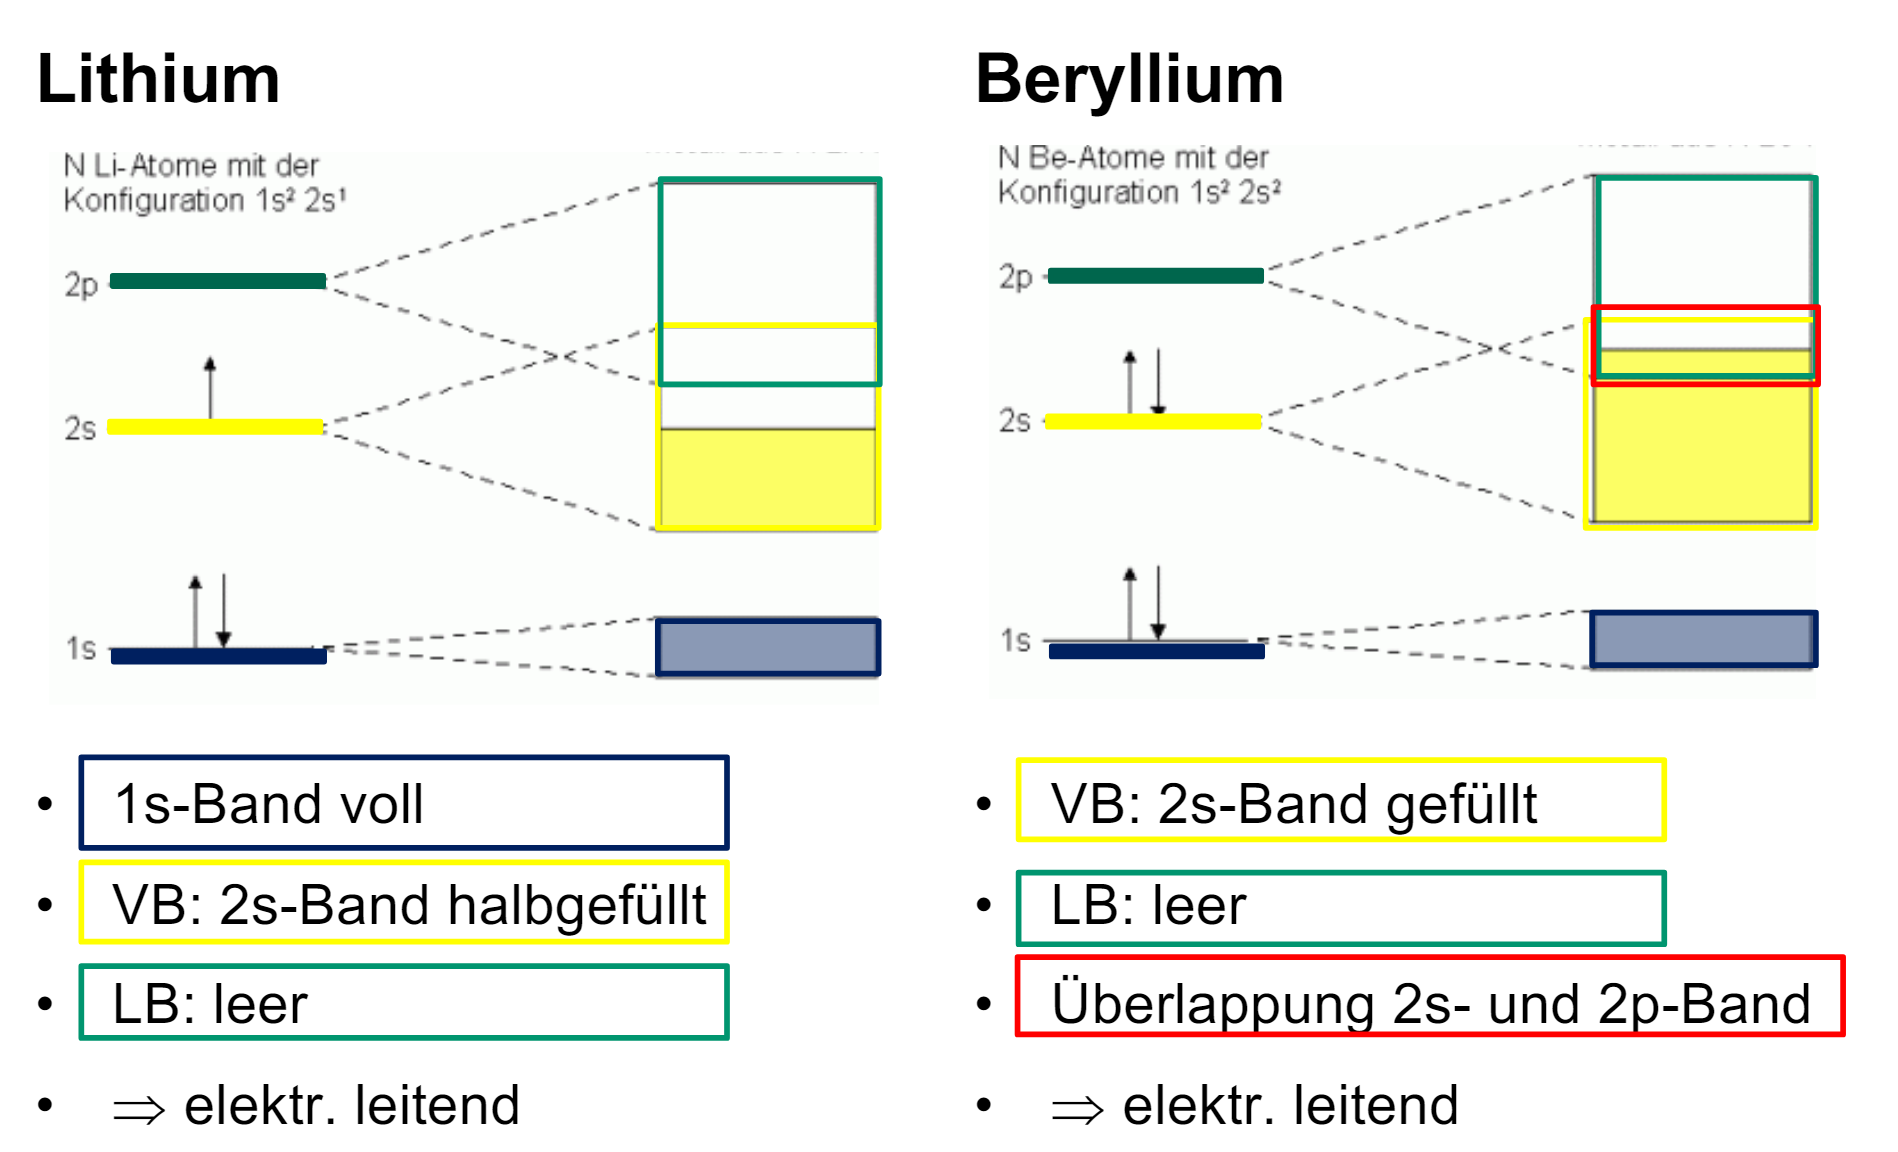
\includegraphics[height=3cm]{pictures/Baender.png}
    \end{center}
    Halbmetalle haben weder Elektronenwolken noch überlappende Energieniveaus, Nähe vom Valenz- und Leitungsband ermöglichen aber ein Überspringen
    \begin{itemize}
        \item Leitfähigkeit bei Halbmetallen 
        \begin{itemize}
            \item nimmt mit steigender Temperatur stark zu
            
                $\rightarrow$ Die Elektronen springen viel zahlreicher auf das Leitungband über
                
                $\Rightarrow$ Platz für Elektronenbewegung im Leitungsband
        \end{itemize}
    \end{itemize}
    % Metalle besitzen durch delokal. Ve (Elektronenwolke) freie Ladungsträger $\rightarrow$ gute Wärme- und el. Leitfähigkeit, Verformbarkeit
    % \begin{itemize}
    %     \item Leitfähigkeit nimmt mit steigender Temperatur ab.\\Die Bewegung der Atomrümpfe erhöht sich wodurch weniger Platz für die ELektronen um sich zu bewegen bleibt.
    % \end{itemize}
    % Allgemein sind Stoffe leitfähig wenn sie entweder wie Lithium:
    % \begin{itemize}
    %     \item das Valenzband (spez. Energieniveau) nicht ganz gefüllt haben und sich dadurch ELektronen in jenem Band bewegen können.
    % \end{itemize}
    % oder wenn sie wie Beryllium:
    % \begin{itemize}
    %     \item das Valenzband komplett gefüllt haben dieses jedoch mit einem leeren Leitungsband überlappt. Wodurch wiederum die beweglichkeit der Elektronen gewährleistet ist.
    % \end{itemize}
    % Halbmetalle haben weder Elektronenwolken noch überlappende Energieniveaus jedoch sind Valenz- und Leitungsband so nahe bei einander das ein überspringen ermöglicht wird.
    % \begin{itemize}
    %     \item Leitfähigkeit nimmt mit zunehmender Temperatur stark zu.\\Die Elektronen springen viel zahlreicher auf das Leitungband über wodurch im Leitungsband wiederum Platz für Elektronenbewegung geschaffen wird.
    % \end{itemize}

\subsection{Dotierung von Halbmetallen}
    Dotierung $\rightarrow$ Einbringen von Fremdatomen ins Atomgitter eines Halbleiters
    \begin{itemize}
        \item \textbf{n-Halbleiter}
        \item[] z.B. einzelne As-Atome im Si-Gitter(1:10'000'000)
        \item[] Ein \textit{überschüssiges} Elektron pro As-Atom $\Rightarrow$ Leitfähigkeit: Elektron von As-Atom kann ins Leitungsband von Si überspringen und sich frei bewegen
        \item \textbf{p-Halbleiter}
        \item[] z.B. einzelne B-Atome im Si-Gitter(1:1'000'000)
        \item[] Ein \textit{fehlendes} Elektron pro B-Atom $\Rightarrow$ Leitfähigkeit: Elektronen aus dem vollen Valenzband von Si können in diese ``Lücke'' springen und sich frei bewegen
    \end{itemize}
\subsection{Bindungswinkel}
    \begin{center}
    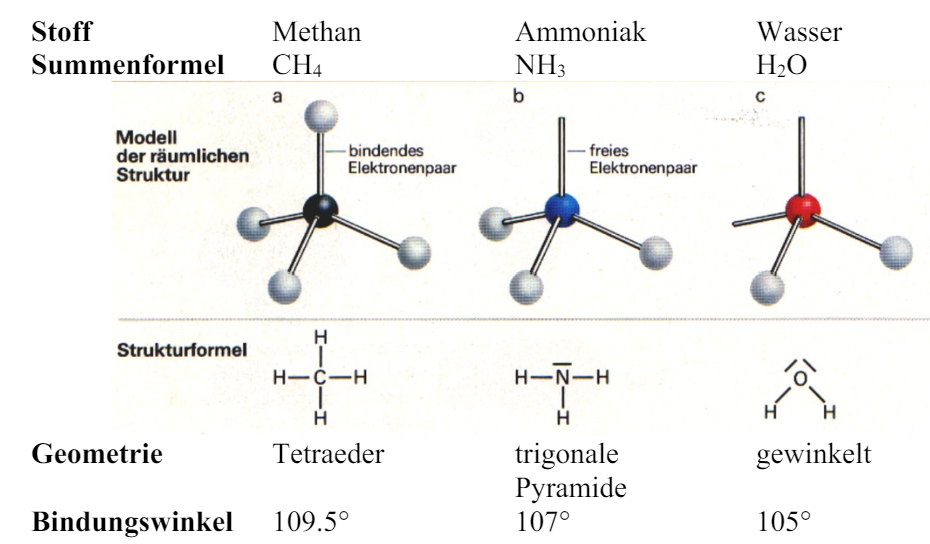
\includegraphics[height=4cm]{pictures/Winkel.png}
    \end{center}

\subsection{Zwischenmolekularkräfte ZMK}
    \begin{itemize}
        \item ... beinflussen Schmelzp., Siedep., Löslichkeit, Viskosität, Oberflächenspannung, ...
        \item Van der Waals (asymm. $e^-$-Verteilung, abh. Anzahl $e^-$) \textcolor{red}{sehr schwach}
        \item Dipol-Dipol (Partialladung, $\delta^+, \delta^-$, $\Delta$EN) \textcolor{orange}{schwach}
        \item Wasserstoffbrücken (H-F-, H-O- oder H-N-Bindungen) \textcolor{green!80!black}{stark}
    \end{itemize}

\subsection{Löslichkeit}
    Die Löslichkeit von Salzen hängt von ihrer Bildungsstärke ab. Je grösser die Ladung der Ionen und je grösser die Ionen, desto schlechter sind sie in Wasser löslich.
    \begin{center}
    \includegraphics[height=2cm]{pictures/Löslichkeit.png}
    \end{center}
        \input{Sections/03_Flüssigkristalle}
        \section{Ablauf chemischer Reaktionen (Freiwilligkeit)}

\subsection{Enthalpie H / Reaktionsenthalpie (Wärme) $\Delta H_R$}
    Prinzip Energieminimum: Stoff will energiearmen Zustand erreichen!

    $\Delta H_R = H_{Produkte} - H_{Edukte} \quad [H] = \frac{\kilo\joule}{\mol \cdot \kelvin}$

    $\Delta H_R < 0 \Rightarrow$ \textcolor{red}{exotherm} $\qquad \Delta H_R > 0 \Rightarrow$ \textcolor{blue}{endotherm}

\subsection{Entropie S (Unordnung) / Reaktionsentropie $\Delta S_R$}
    Prinzip Energiemax: alle Stoffe und Systeme wollen möglichst grosse Entropie

    $\Delta S_R = \sum S^0_{Produkte} - \sum S^0_{Edukte} \qquad \qquad [\Delta S_R] = \frac{\color{red}\joule}{\mol \cdot \kelvin}$

    $S^0$: Molare Standartentropie (1mol des Stoffs bei Std.Bedingungen)
\subsection{Freie Enthalpie $\Delta G$}
    Beschreibt Freiwilligkeit der Reaktion:

    $\Delta G = \Delta H - T \cdot \Delta S \qquad \qquad [\Delta G] = \frac{\kilo\joule}{\mol}$

    $\Delta G < 0:$ Exergon (freiwillige Reaktion) $\qquad \Delta G > 0:$ Endergon(unfreiwillige Reaktion)

    % \begin{itemize}
    %     \item $\Delta G < 0:$ Exergon (freiwillige Reaktion)
    %     \item $\Delta G > 0:$ Endergon(unfreiwillige Reaktion)
    % \end{itemize}

\subsection{Aktivierungsenergie/Reaktionsgeschw./Katalysatoren}
\begin{minipage}{0.32\linewidth}
    % \vspace*{0pt}
    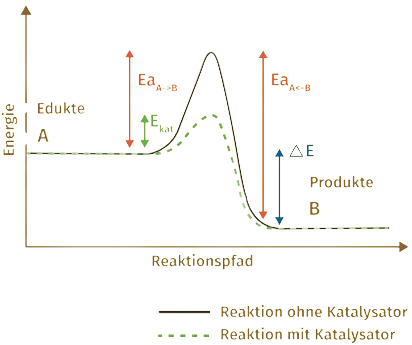
\includegraphics[width=\linewidth]{pictures/Katalysator_1.png}
\end{minipage}
\hfill
\begin{minipage}{0.65\linewidth}
    \begin{itemize}
        \item RGT-Regel: $\Delta$ T = 10 $\rightarrow$ RG $\cdot$ 2
        \item Katalysator = Stoff nimmt an Reaktion teil, wird nicht verbraucht 
        \item Beschleunigt Reaktion: $E_{AKat} \ll E_{ANorm}$
        \item $\Delta$ G sowie $\Delta H_R$ bleiben gleich
        \item Selektiv (wirkt nicht mit allen Stoffen)
    \end{itemize}
\end{minipage}

        \input{Sections/05_Säure-Base-Reaktionen}
        \section{Redox-Reaktionen}

\subsection{Grundlagen}
    Eine Reaktion ist eine Redox-Reaktion, wenn die Oxidationszahlen der Atome der Edukte nicht die selben sind wie die Oxidationszahlen der Atome der Produkte.
    \begin{center}
        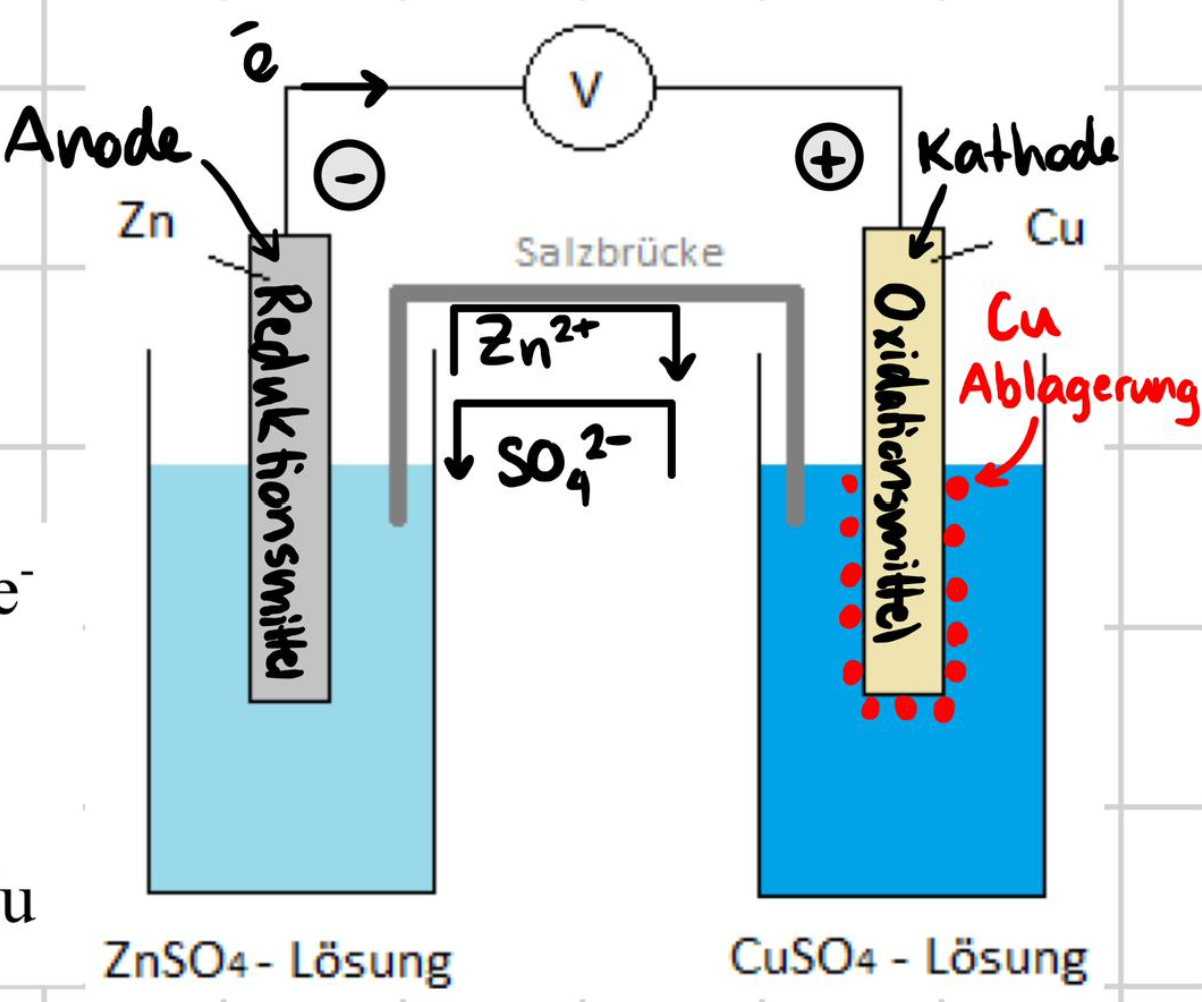
\includegraphics[height=4cm]{pictures/Galv.png}
    \end{center}
    Aufgrund der \textbf{Standartpotenziale} der Metalle Zn und Cu herrscht eine ``Spannun'', welche die Reaktion ermöglicht. 
    Das \textbf{\ce{Zn^0}} wird an der Anode zu \textbf{\ce{Zn^2+}} oxidiert (\ce{e^-}-Abgabe), \textbf{\ce{Zn^0}} dient somit als Reduktionsmittel. 
    Die Elektronen werden an die Kathode abgegeben, wo \textbf{\ce{Cu^2+}} aus der Lösung zu \textbf{\ce{Cu^0}} reduziert (\ce{e^-}-Aufnahme) wird. 
    \textbf{\ce{Cu^2+}} dient somit als Oxidationsmittel. Damit die Lösungen jeweils ungeladen bleiben, wandern über die Salzbrücke 
    \textbf{\ce{Zn^2+}-Ionen} und \textbf{\ce{SO4^2-}-Ionen}.
\subsection{Redoxpotential}
    Das Redoxpotential einer Halbzelle kann aus der Redox-Reihe ausgelesen werden (ganz rechts). Dieses Potenzial wurde jeweils 
    gegenüber einer Standart-Wasserstoff-Elektrode gemessen.
    
    Das Redoxpotential ist jedoch von pH, Druck, Ionenkonz und Temperatur abhängig. Potenziale bei Nicht-Standardbedingungen können 
    mit folgender GLeichung berechnet werden.

    Nernst-Gleichung:\\
    \begin{minipage}{0.4\linewidth}
        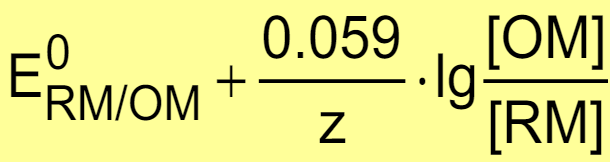
\includegraphics[width=\linewidth]{pictures/Nernst.png}
    \end{minipage}
    \hfill
    \begin{minipage}{0.55\linewidth}
        \begin{itemize}
            \item z = Anz. \ce{e^-} die pro Atom übergeben werden
            \item \ce{[OM]} = konz. OM in mol/L
            \item \ce{[RM]} = konz. RM in mol/L
        \end{itemize}
    \end{minipage}

    \begin{center}
        Inkl. pH-Wert:\\
        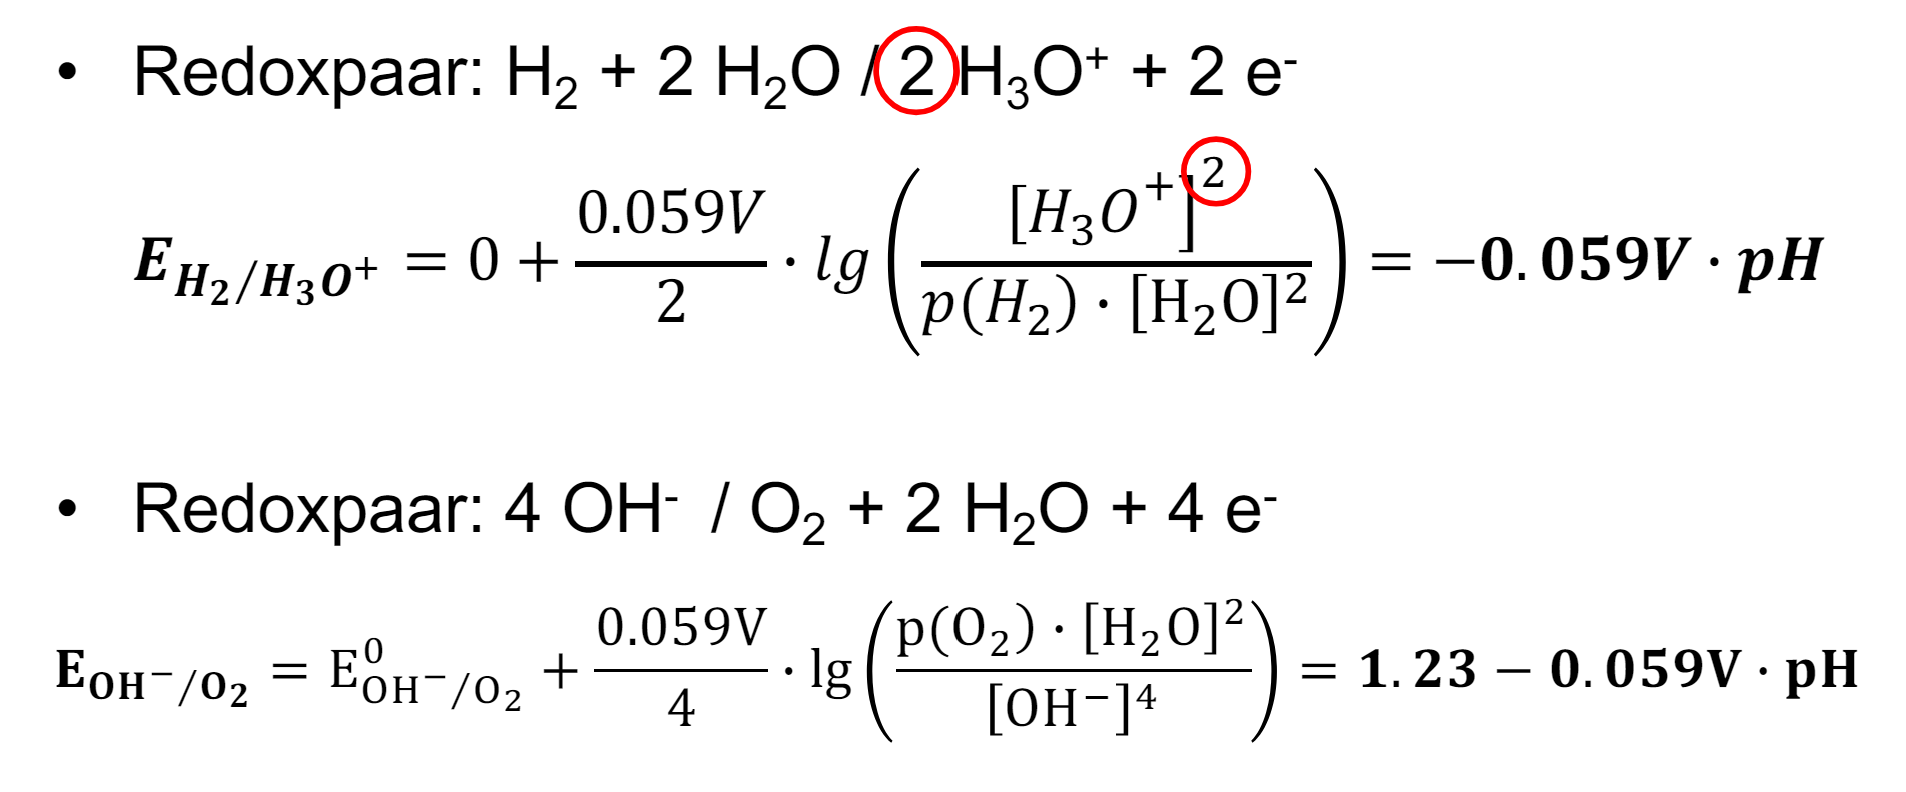
\includegraphics[height=3cm]{pictures/Nernstph.png}
    \end{center}
        \section{Anwendungen der Redox-Reaktionen}
   Spannung galvanische Zelle: $U = \ce{E^{Kathode}} - \ce{E^{Anode}} V$
% TODO: mehr einfügen, ansonsten killen

        \section{Korrosion}
    Metall reagiert als RM: \ce{Me <--> $Me^{z+}$ + z e-}
    
    Möglich wenn $\Delta$G $<$ 0 $\&$ v.a. \ce{O2, H2O/H3O+} (OM) vorhanden

\subsection{Korrosionsarten}
    \subsubsection{Elchem Korrosion}
        $\Rightarrow$ Bildung galvanische Zelle
    \subsubsection{O2-Typ-Korrosion}
        \ce{O2 + 2H2O + 4e- -> 4OH-}\\
        \ce{2Fe + 3/2 O2 + H2O -> 2FeOOH}\\
        Voraussetzung ist Vorhandensein von \ce{O2} und \ce{H2O}; RG relativ langsam!
    \subsubsection{Säure/Wasserstoffkorrosion}
        Ist pH-Abhängig:
        \begin{itemize}
            \item Sauer: \ce{2H3O+ + 2 e- <--> H2 + 2H20}
            \item Basisch: \ce{2H2O + 2 e- <--> H2 + 2 OH-}
        \end{itemize}
    \subsubsection{Beispiele Al H-Typ-Korrosion}
        \textbf{H2 Korrosion von Al in basischer Lösung}\\
        \begin{tabular}{p{1.8cm}ccc}
            Depassivierung: & \ce{Al2+2OH-+3H2O}        & \ce{->} & \ce{2[AL(OH)4]-(aq)}\\
            Oxidation:      & \ce{Al}                   & \ce{->} & \ce{Al3+ + 3e-}\\
            Reduktion:      & \ce{2H2O + 2 e-}          & \ce{->} & \ce{H2 + 2OH-}\\
            Redoxreaktion:  & \ce{2 Al + 6 H2O + 2OH-}  & \ce{->} & \ce{2[Al(OH)4]- + 3H2}
        \end{tabular}

        \textbf{H2 Korrosion von Al in saurer Lösung}\\
        \begin{tabular}{p{1.8cm}ccc}
            Oxidation:      & \ce{Al}               & \ce{->} & \ce{Al3+ + 3e-}\\
            Reduktion:      & \ce{2H3O+ + 2e-}      & \ce{->} & \ce{H2 + H2 + 2 H2O}\\
            Redoxreaktion:  & \ce{2 Al + 6 H3O+}    & \ce{->} & \ce{2 Al3+ + 6H2O + 3H2}
        \end{tabular}
\subsection{Oxidschichten}
    Metallische Werkstoffe (ausser Gold/Platinmetalle) bilden bei Raumtemperatur mit Luft eine Oxidschicht, es entsteht ein Metalloxid:\\
    \ce{n Me + \frac{m}{2} O2 -> $Me_nO_m$}\\
    Der Schutzfaktor kann mittels PBV ermittelt werden:\\
    $PBV = \frac{V(Metalloxid)}{V(Metall)}$\\
    \begin{itemize}
        \item PBV $\ll$ 1: Rissige, nicht schützende Schicht (MG(0.8), Na (0.3))
        \item PBV 1- 2: Kompakte, schützende Oxidschicht (Al(1.3), Ni(1.5), Ti(1.7), Cu(1.7), Cr(2.1), Fe(2.1))
        \item PBV $\gg$ 2: Abblätternde nicht schützende Schicht (V(3.2), W(3.4), Rost(3.6))
    \end{itemize}
\subsection{Ablauf der Korrosion in wässrigen Lösungen}
    Alle Korrosionsreaktionen verlaufen in 2 Teilschritten:
    \begin{itemize}
        \item Depassivierung
        \item Eigentliche Korrosion
    \end{itemize}

    Voraussetzungen für Korrosion:
    \begin{itemize}
        \item Metall ist in Elektrolytlösung eingetaucht
        \item Metall ist von dünnem Flüssigkeitsfilm bedekt.\\
        Können durch Regen, Tau, Bodenfeuchtigkeit oder rel. Luftfeuchtigkeit $> 70\%$ entstehen. Bei Oberflächen mit hygroskopischen Salzen kann auch früher Korrosion entstehen.
    \end{itemize}
\subsection{Passivatoren und Depassivatoren}
    Depassivierung hängt vom Gehalt von Passivatoren und Depassivatoren in Elektrolytlösung ab
    \subsubsection{Passivatoren}
        $\Rightarrow$ bieten \textbf{anodischen Schutz}($E_A$ wird vergrössert)
        \begin{itemize}
            \item Fe: \ce{OH-, CrO4^{2-}, NO2-}
            \item Al: \ce{NO3-}
        \end{itemize}
        
    \subsubsection{Depassivatoren}
        $\Rightarrow$ \textbf{zerstören Passivoxidfilm}, bewirken (oft lokale \textbf{Depassivierung}($E_A$ wird verkleinert))
        \begin{itemize}
            \item Fe: \color{blue} \ce{Cl-}\color{black}, \color{red} \ce{H3O+}\color{black}, \ce{SO4^2-}
            \item Al: \color{blue} \ce{Cl-}\color{black}, \color{red} \ce{H3O+}\color{black}, \ce{OH-}
            \item Cu: \color{blue} \ce{Cl-}\color{black}, \color{red} \ce{H3O+}\color{black}, \ce{NH3}
            \item Ni: \color{blue} \ce{Cl-}\color{black}, \color{red} \ce{H3O+}\color{black}
        \end{itemize}
        
\subsection{Potentialverhältnisse/Aktivierungsenergie}
    Wann korrodieren Metalle nach \ce{H2}/\ce{O2}-Typ?\\
    $\Rightarrow \Delta$G $<$ 0\\
    $\Rightarrow$ Korrosion abhängig von E(M/\ce{M^z+}) unsd E(OM)\\
    E(OM) ist pH-abhängig:\\
    $E_{H2}$ = -0.059*pH\\
    $E_{O2}$ = 1.23 - 0.059*pH\\
\subsection{Kontaktkorrosion}
    \begin{itemize}
        \item Reduktion von \ce{O2} an gesamter Oberfläche
        \item Oxidation nur an unedlerem Metall $\rightarrow$ verstärkte Korrosion
        \item Edleres Metall $\rightarrow$ keine Korrosion(kathodisch geschützt)
        \item Flächenregel: $\frac{v_k(Zn)}{v_k(Zn + Fe)} = \frac{A(Zn)}{A(Zn + Fe)}$
    \end{itemize}

\subsection{Lochfrasskorrosion}
    \begin{itemize}
        \item Stark lokalisierte Korrosion
        \item Bildung enger tiefer Löcher
        \item schwer erkennbar
    \end{itemize}

\subsection{Belüftungselemente}
    \begin{itemize}
        \item Kann nur bei passivierbaren Metallen auftreten!
        \item Für Passivschicht ist \ce{O2} notwendig
        \item An engen Stellen kann \ce{O2}-Zufuhr erschwert werden $\rightarrow$ Depassivierung $\Rightarrow$ Lochfrass
        \item Zusätzlich Flächenregel (Spalt $\rightarrow$ kleine Anode, Passivoxidschicht $\rightarrow$ grosse Kathode)
    \end{itemize}


        
        \section{Emotional support meme}
        \begin{center}
            
\includegraphics[width=\columnwidth]
            {pictures/argon.jpeg} 
        \end{center}

    \end{layout}	
\end{document}
